{\actuality} Магнитоэлектрические эффекты обусловлены наличием в термодинамическом потенциале членов, линейных как по электрическому, так и по магнитному полю \autocite{Landau}. Данные эффекты наблюдаются в магнитоэлектриках и мультиферроиках в случае, когда одновременно нарушается симметрия относительно обращения знака времени (следствие магнитного упорядочения) и симметрия относительно пространственной инверсии (следствие особенностей кристаллической структурой) - магнитными свойствами этих материалов можно управлять прикладывая внешнее электрическое поле и наоборот. Так, авторы работы \autocite{Saito2008ape} наблюдали в антиферромагнетике \cbo\ вращение намагниченности, индуцированное электрическим полем. Позднее другая группа смогла управлять электрической поляризацией \ncbo\ с помощью внешнего магнитного поля \autocite{Khanh2013}. Кроме описанных \emph{статических} магнитоэлектрических эффектов существуют также \emph{динамические} - связанные с взаимодействием с периодическими электромагнитными полями. В частности, к таковым относятся явление невзаимности (nonreciprocity) в спектрах поглощения \autocite{Toyoda2015} и явление пространственной асимметрии люминесценции (directional asymmetry of luminescence) \autocite{Toyoda2016}.  

Интерес к этим эффектам в последние десятилетия существенно возрос, в связи с реальными перспективами практических применений. На основе магнитоэлектрических материалов можно создавать магнитные запоминающие устройства с оптическим считыванием информации о доменной структуре, управляемые магнитным полем оптические диоды и пр. (см. рисунок \cref{fig:applications}) Также, разумеется, изучение данных эффектов важно для фундаментальных научных исследований.

\begin{figure}[ht]
	\centerfloat{
		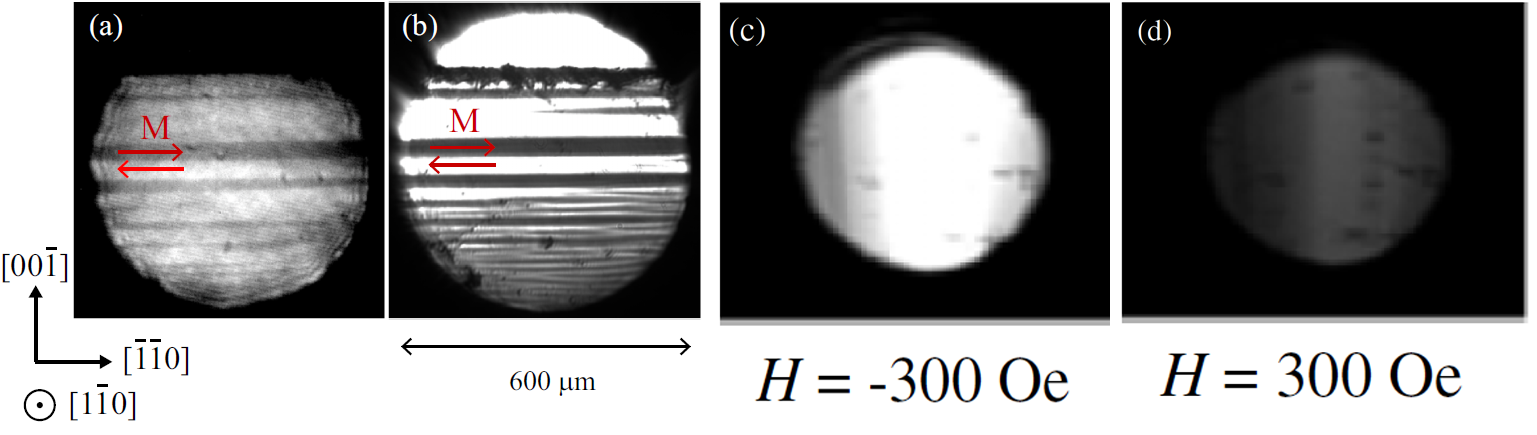
\includegraphics[scale=0.4]{applications}
	}
	\caption{(a), (b) Фотографии магнитных доменов из \autocite{Toyoda2016}, полученные с помощью фотолюминесценции. (c), (d) Фотографии света, прошедшего через пластинку \cbo\, к которой приложили внешнее магнитное поле в -300 и 300~Э~\autocite{Saito2008jpsj}. (a, b) и (c, d) сделаны при одной и той же яркости и контрасте.}\label{fig:applications}
\end{figure}

Можно выделить два подхода в развитии теории магнитоэлектрических эффектов: феноменологический и микроскопический. Феноменологический подход сформулирован в работе Дзялошинского \autocite{Dzyaloshinskii1959}. Этот подход успешно использовался для анализа ряда материалов. Его применение описано во многих обзорах и оригинальных статьях \autocite{Zvezdin2008, Pyatakov2012, Popkov2016}. Микроскопический подход развит слабее и предполагает предварительный анализ энергетических схем уровней и взаимодействий магнитных ионов с обменными и электрическими полями.

{\aim} данной работы является разработка микроскопической теории статических и динамических магнитоэлектрических эффектов в диэлектрике \cbo\ на основе квантово-механического подхода.

Для~достижения поставленной цели необходимо было решить следующие {\tasks}:
\begin{enumerate}[beginpenalty=10000] % https://tex.stackexchange.com/a/476052/104425
	\item проанализировать и систематизировать имеющиеся на момент написания работы данные по экспериментальному наблюдению и теоретическому описанию магнитоэлектрических эффектов в \cbo;
	\item получить уровни энергии и волновые функции иона меди 3d\(^9\) в кристалле \cbo
	\item оценить параметры взаимодействия электронов меди с электрическим и магнитным полем
	\item сопоставить результаты теоретических расчетов с имеющимися экспериментальными данными
\end{enumerate}


{\novelty}
\begin{enumerate}[beginpenalty=10000] % https://tex.stackexchange.com/a/476052/104425
	\item Как это подчеркивается в обзорах \autocite{Khomskii2009, Moskvin2009, Tokura2014, Shuai2015}, микроскопические механизмы магнитоэлектрической связи еще не вполне выяснены.
	\item Впервые построены теоретические диаграммы пространственной асимметрии люминесценции, которые не могут быть получены в рамках теоретико-группового подхода.
	\item Получен эффективный оператор статической магнитоэлектрической связи, отличный от используемых ранее для объяснения электрической поляризации в \ncbo.
\end{enumerate}


{\probation}
Основные результаты работы докладывались~на:
\begin{enumerate}[beginpenalty=10000] % https://tex.stackexchange.com/a/476052/104425
	\item \textit{Нурмухаметов, А. Р.} Особенности экситонных зон Френкеля-Давыдова в антиферромагнетиках [Устный доклад] / А.~Р.~Нурмухаметов // Итоговая конференция Института Физики. - 2021.
	\item \textit{Нурмухаметов, А. Р.} Магнитоэлектрическая связь в Cu\(_{1-x}\)Ni\(_{x}\)B\(_{2}\)O\(_{4}\) [Устный доклад] / А.~Р.~Нурмухаметов // Итоговая конференция Института Физики. - 2022.
	\item \textit{Нурмухаметов, А. Р.} К теории необратимости в спектрах \cbo\ [Стендовый доклад] / А.~Р.~Нурмухаметов, М.~В.~Еремин // Нанофизика и наноэлектроника. Труды XXVI Международного симпозиума. - 2022.
\end{enumerate}


\ifnumequal{\value{bibliosel}}{0}
{%%% Встроенная реализация с загрузкой файла через движок bibtex8. (При желании, внутри можно использовать обычные ссылки, наподобие `\cite{vakbib1,vakbib2}`).
    {\publications} Основные результаты по теме диссертации изложены
    в~XX~печатных изданиях,
    X из которых изданы в журналах, рекомендованных ВАК,
    X "--- в тезисах докладов.
}%
{%%% Реализация пакетом biblatex через движок biber
    \begin{refsection}[bl-author, bl-registered]
        % Это refsection=1.
        % Процитированные здесь работы:
        %  * подсчитываются, для автоматического составления фразы "Основные результаты ..."
        %  * попадают в авторскую библиографию, при usefootcite==0 и стиле `\insertbiblioauthor` или `\insertbiblioauthorgrouped`
        %  * нумеруются там в зависимости от порядка команд `\printbibliography` в этом разделе.
        %  * при использовании `\insertbiblioauthorgrouped`, порядок команд `\printbibliography` в нём должен быть тем же (см. biblio/biblatex.tex)
        %
        % Невидимый библиографический список для подсчёта количества публикаций:
        \printbibliography[heading=nobibheading, section=1, env=countauthorvak,          keyword=biblioauthorvak]%
        \printbibliography[heading=nobibheading, section=1, env=countauthorwos,          keyword=biblioauthorwos]%
        \printbibliography[heading=nobibheading, section=1, env=countauthorscopus,       keyword=biblioauthorscopus]%
        \printbibliography[heading=nobibheading, section=1, env=countauthorconf,         keyword=biblioauthorconf]%
        \printbibliography[heading=nobibheading, section=1, env=countauthorother,        keyword=biblioauthorother]%
        \printbibliography[heading=nobibheading, section=1, env=countregistered,         keyword=biblioregistered]%
        \printbibliography[heading=nobibheading, section=1, env=countauthorpatent,       keyword=biblioauthorpatent]%
        \printbibliography[heading=nobibheading, section=1, env=countauthorprogram,      keyword=biblioauthorprogram]%
        \printbibliography[heading=nobibheading, section=1, env=countauthor,             keyword=biblioauthor]%
        \printbibliography[heading=nobibheading, section=1, env=countauthorvakscopuswos, filter=vakscopuswos]%
        \printbibliography[heading=nobibheading, section=1, env=countauthorscopuswos,    filter=scopuswos]%
        %
        \nocite{*}%
        %
        {\publications} Основные результаты по теме диссертации изложены в~\arabic{citeauthor}~печатных изданиях,
        \arabic{citeauthorvak} из которых изданы в журналах, рекомендованных ВАК\sloppy%
        \ifnum \value{citeauthorscopuswos}>0%
            , \arabic{citeauthorscopuswos} "--- в~периодических научных журналах, индексируемых Web of~Science и Scopus\sloppy%
        \fi%
        \ifnum \value{citeauthorconf}>0%
            , \arabic{citeauthorconf} "--- в~тезисах докладов.
        \else%
            .
        \fi%
        \ifnum \value{citeregistered}=1%
            \ifnum \value{citeauthorpatent}=1%
                Зарегистрирован \arabic{citeauthorpatent} патент.
            \fi%
            \ifnum \value{citeauthorprogram}=1%
                Зарегистрирована \arabic{citeauthorprogram} программа для ЭВМ.
            \fi%
        \fi%
        \ifnum \value{citeregistered}>1%
            Зарегистрированы\ %
            \ifnum \value{citeauthorpatent}>0%
            \formbytotal{citeauthorpatent}{патент}{}{а}{}\sloppy%
            \ifnum \value{citeauthorprogram}=0 . \else \ и~\fi%
            \fi%
            \ifnum \value{citeauthorprogram}>0%
            \formbytotal{citeauthorprogram}{программ}{а}{ы}{} для ЭВМ.
            \fi%
        \fi%
        % К публикациям, в которых излагаются основные научные результаты диссертации на соискание учёной
        % степени, в рецензируемых изданиях приравниваются патенты на изобретения, патенты (свидетельства) на
        % полезную модель, патенты на промышленный образец, патенты на селекционные достижения, свидетельства
        % на программу для электронных вычислительных машин, базу данных, топологию интегральных микросхем,
        % зарегистрированные в установленном порядке.(в ред. Постановления Правительства РФ от 21.04.2016 N 335)
    \end{refsection}%
    \begin{refsection}[bl-author, bl-registered]
        % Это refsection=2.
        % Процитированные здесь работы:
        %  * попадают в авторскую библиографию, при usefootcite==0 и стиле `\insertbiblioauthorimportant`.
        %  * ни на что не влияют в противном случае
        \nocite{vakbib2}%vak
        \nocite{patbib1}%patent
        \nocite{progbib1}%program
        \nocite{bib1}%other
        \nocite{confbib1}%conf
    \end{refsection}%
        %
        % Всё, что вне этих двух refsection, это refsection=0,
        %  * для диссертации - это нормальные ссылки, попадающие в обычную библиографию
        %  * для автореферата:
        %     * при usefootcite==0, ссылка корректно сработает только для источника из `external.bib`. Для своих работ --- напечатает "[0]" (и даже Warning не вылезет).
        %     * при usefootcite==1, ссылка сработает нормально. В авторской библиографии будут только процитированные в refsection=0 работы.
}

